\documentclass{standalone}
\usepackage{pgfplots}
\pgfplotsset{compat=1.8}

\begin{document}

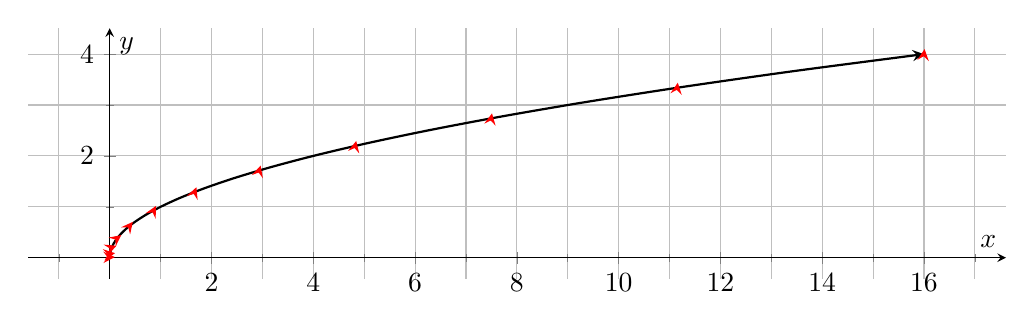
\begin{tikzpicture}
\begin{axis}[
width=14cm,
axis lines = middle,smooth,xlabel = $x$, ylabel =$y$, minor tick num =1, grid=both, unit vector ratio*=1 1,enlargelimits = true]
\addplot[smooth, thick, -stealth,variable=\t, domain=0:2]
    ({t^4}, {t^2});

\def\NORM{sqrt((2*t)^2 + (4*t^3)^2)}
\addplot[thick, red,-stealth,samples=12,variable=\t, domain=0.1:2,quiver={
        u=2*t/\NORM, v=4*t^3/\NORM,
        scale arrows=0.1,
    }]
    ({t^4}, {t^2});
\end{axis}
\end{tikzpicture}

\end{document}
